\documentclass{article}
\usepackage{amsmath,amssymb,amsbsy,amsfonts,amsthm}
\usepackage{graphics,epsfig,graphicx,float,subfigure,color}

\title{Reinforcement Learning Under Uncertainty}
\author{Abraham Frei-Pearson \\
	Department of Mathematics  \\
	\and 
	Sheroze Sheriffdeen \\
	Oden Institute \\
	}

\date{\today}
% Hint: \title{what ever}, \author{who care} and \date{when ever} could stand 
% before or after the \begin{document} command 
% BUT the \maketitle command MUST come AFTER the \begin{document} command! 
\begin{document}

\maketitle
\section{Introduction and Related Work}
In this project, we are interested in applying reinforcement learning techniques to noisy optimal control problems. The general case will be in the following form. Given an unknown matrix $A \in \mathbb{R}^{n \times n}$, and evolution of state $x_t \in \mathbb R^n$ governed by dynamics
\[
    x_{t+1} = (I + A(x_t)) x_t + u(x_t) + g,
\]
where $g$ is Gaussian noise, how does one learn the control function $u$ so as to minimize $J = \sum_{t=0}^{T} \left[ || x_t ||_U + || u(x_t)||_O \right]$, where $U$ and $O$ define norms in the state space and the control space respectively? There are several abstractions we are interested in considering: noise in the system itself, noise in the observations of the state, and noise in the reward function. 

Noisy dynamics introduce maximization bias, as discussed in Sutton and Barto~\cite{suttonAndBarto}, into the standard reinforcement learning algorithms. Early in training, noise causes the best-looking action to look better than it actually is. This is dealt with effectively by double-Q learning. Another algorithm for dealing with maximization bias is discussed in \cite{foxPakmanTishby}, dubbed "G-learning". This algorithm begins with a stochastic policy $\rho$. A pseudo-reward is calculated for each state action pair called $G_\pi(s,a)$, where $G_\pi(s,a)$ is $Q(s,a)$ less an information cost which is a discounted version of the Kullback-Liebler divergence $KL(\pi( \dot , s) || \rho( \dot , s))$.

In the case of traditional optimal control, at least when the state dynamics are locally linear, an optimal estimate for the state is given by extended Kalman filtration~\cite{welchBishop}. This is optimal in the sense that, given knowledge about the noise, the Kalman estimate for the state minimizes the expected squared error. The Kalman estimate is as follows: suppose the matrix $A$ above is known, and our current estimate for $x_t$ is $\hat x_t^p$. We choose control variables, or actions, based on this estimate and obtain a new reward and state observation. We update our estimate of the state based on the current observations by computing $K$m the {\em Kalman gain}, obtained by minimizing the a posteriori variance of the estimate. We would like to see how applying the Kalman filter to our observation data in a noisy environment improves the usual reinforcement learning methods compared to acting directly on measurements. Although we need a model to apply the Kalman filter, it would still be interesting to study improvements to reinforcement learning from filtered data. 

\subsection{Related Work}
Kalman filtration is applied to reinforcement learning problems in~\cite{trippSchacter} in a somewhat different way. In this case it  is applied to the update of the $Q$-function directly, and then $Q$-learning is applied. Kalman temporal differencing~\cite{geist2010kalman} shows another approach where value function approximation is cast as a filtering problem in order to benefit from online second order learning, uncertainty estimation and non-stationarity handling. 

Kalman filtering is also applied to dynamical systems with unknown dynamics. Consider the case where matrix $A$ is unknown a priori in the discrete linear dynamical system with noise
\[
    x_{t+1} = (I + A) x_t + \eta +  u_t x_t,
\]
where $\eta$ is Gaussian and $u_t$ is a linear control and reward is defined to be $1$ for all $t$ where $x_t$ is within a ball around the origin. This problem is studied in ~\cite{ornikIsraelTopcu} and \cite{ahmadiIsraelTopcu}, using the theory of differential inclusions. This is also addressed in~\cite{bagnell2004policy} in the min-max setting. Given a set of transitions $\mathcal P$, an algorithm for producing a policy maximizing $\mathbb E_{p \in \mathcal P, \Pi} \sum\limits_t \gamma^t R(X_t)$, where $X_t$ is the trajectory under $\pi$, is presented. This algorithm could be adjusted to include a prior on the transitions, and optimize the expected reward according to that prior rather than the min-max reward. 

A reformulation of the stochastic optimal control problem in terms of KL divergence minimization is examined by Rawlik et. al \cite{rawlik2013stochastic}. This work considers reinforcement learning as an instance of stochastic optimal control which does not assume knowledge of the dynamics.  A cost is associated with each policy relating to a measure of the control, and the stochastic optimal policy is posed as finding an optimal policy that minimizes the expected cost of controls following trajectories under the given policy. An experiment performed with the cart-pole problem with zero mean Gaussian noise added to the state and an extended Kalman smoother \cite{stengel1986stochastic} is use to estimate a Gaussian approximation to the full posterior of the state variables, leading to a Gaussian posterior policy.


\section{G-learning}

\subsection{Description of the algorithm}

We begin by recalling the setup for $Q$-learning. For consistency with ~\cite{foxPakmanTishby}, we will state the algorithm in terms of costs rather than rewards. For an MDP with discount $\gamma$, a state-action value function $Q$, and an observed state, action, cost, and new state $s,a,c,s'$, we perform the update $Q(s,a)=\alpha Q(s,a) + (1-\alpha) (c + \gamma \arg \min\limits_{a'} Q(s',a))$. Action are chosen according to a policy which is $\epsilon$ greedy with respect to $Q$.

Although there are robust convergence guarantees for $Q$-learning, in the presence of noise $Q$-learning converges very slowly. The reason is this: suppose that, early in training, we observe a particularly low value of $Q(s,a)$ early in training due to stochasticity. Then, with high probability, the action $a$ will be chosen whenever the MDP is in the state $s$, preventing exploration.

$G$ learning is obtained from $Q$ learning by adding an information cost with respect to a given baseline policy $\rho$. Specifically, $g^\pi(s,a) = \log(\frac{\pi(a | s)}{\rho(a | s)})$. Then the information cost of a state $s$ is
\[
    I^\pi(s) = \sum\limits_{t \geq 0} \gamma^t \mathbb E [g^\pi(s_t,a_t) | s_0 = s].
\]
Set set the state value to be $F^\pi(s) = V^\pi(s) + \frac{1}{\beta} I^\pi(s)$. The number $\beta$ is a parameter which can be tuned to the problem and the baseline policy $\rho$. The state action function $G^\pi(s,a)$ is then defined as
\[
    G^\pi(s,a) = \mathbb E(c|s,a) + \gamma \mathbb E(F^\pi(s')|s,a],
\]
where $c$ is the cost and $F^\pi(s')$ is the state value of the next state. We thus obtain 
\[
    F^pi(s) = \sum\limits_{a} \pi(a|s) (\frac{1}{\beta} \log \frac{\pi(a|s)}{\rho(a|s)} + G^\pi(s,a).
\]
Setting the gradient of this with respect to $\pi(a|s)$ to zero gives
\[
    \pi(a|s) = \frac{\rho(a|s) e^{-\beta G(s,a)}}{\sum\limits_{a'} \rho(a'|s) e^{-\beta G(s,a')}}.
\]
This leads to the update
\[
    G(s,a) \leftarrow (1-\alpha) G(s,a) + \alpha(c - \frac{\gamma}{\beta} \log(\sum\limits_{a'} \rho(a'|s') e^{-\beta G(s',a')})
\]
given the observation $s,a,r,s'$.

The temperature parameter $\beta$ encodes how much preference is given to the prior policy $\rho$. When $\beta$ is small, $G$-learning heavily penalizes policies which are different from $\rho$. In the limit, when $\beta = 0$, $G$-learning will only allow the function $\rho$ to be used. On the other hand, as $\beta \to \infty$, the behavior of $G$-learning tends to that of $Q$-learning. In practice, we set $\beta = i$ for the $i$th episode.

\subsection{Experiment}

We tested the performing of $G$-learning against $Q$-learning in the simple gridworld setup of ~\cite{suttonAndBarto}, example 4.1. Here we have a 4x4 grid with terminal states in the upper left and lower right corners, with a reward of $-1$ (or a cost of $1$) for each transition. We trained a $Q$-learning and a $G$-learning agent on this environment: we ran trained 200 independent agents on $Q$- and $G$-learning each for 40 episodes, and recorded the cumulative score. We took the learning rate $\alpha$ to be $0.1$, the parameter $\epsilon$ in $Q$-learning (the $\epsilon$ with respect to which the policy is $\epsilon$-greedy) to be $0.1$, the prior policy to be uniform at random, and the temperature parameter $\beta$ to be $i$ in the $i$th episode. Note that in all cases $G$-learning outperforms $Q$-learning, but $G$-learning performs even better in the case of greater noise.

In the figure below, the $x$ axis represents the size of the noise term: for each $x$ we added a uniform random variable to the return drawn from $[-x,x]$. The $y$-axis represents the difference in the cumulative reward over the 40 episodes between $Q$-learning and $G$-learning, averaged over all 200 runs.

\begin{figure}[H]
\centering
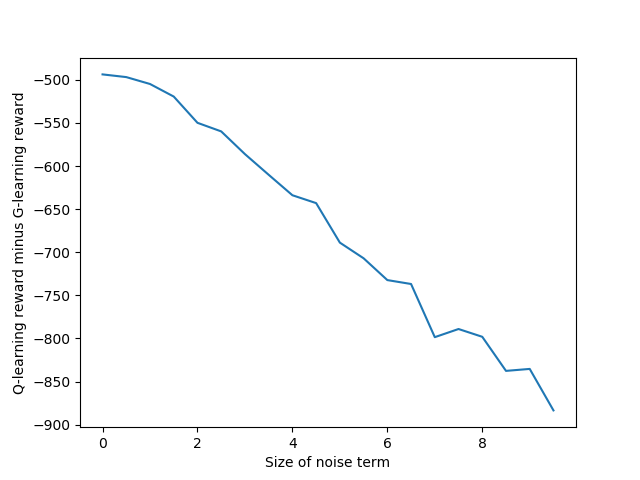
\includegraphics[scale=0.7]{noisevsreward.png}
\end{figure}


\section{Kalman Filtering for State Estimation}
\subsection{Discrete Time-Controlled Processes}

For this section of our project, we are interested in applying reinforcement learning techniques to noisy optimal control problems. The general case will be in the following form. Given matrices $A \in \mathbb{R}^{n \times n}$, $B \in \mathbb{R}^{n \times n_u}$, and the state represented by a vector $x_t \in \mathbb R^n$, our dynamics will be governed by the linear stochastic difference equation
\begin{equation}
    x_{t+1} = (I + \triangle t A) x_t + Bu(x_t) + w_t,
    \label{eq:dynamical}
\end{equation}
with state measurements $z_t \in \mathbb{R}^{n_o}$, 
\[
	z_{t+1} = H x_{t+1} + v_{t+1}
\]
The random variables $w_t$ and $v_t$ represent process and measurement noise respectively. They are assumed to be independent of each other, white, with normal probability distributions
\[ 
p(w) \sim \mathcal{N}(0, Q)
\]
\[
p(v) \sim \mathcal{N}(0, R)
\]
$u(x_t) \in \mathbb{R}^{n_u}$ is the control vector that we are trying to learn using reinforcement learning. We employ true-online TD($\lambda$) to learn a parametrized control vector at each time step given noisy measurements of state.

\subsection{State Estimation with Kalman Filtering}

The following is from the excellent introduction to Kalman filters by Welch and Bishop ~\cite{welchBishop}. The Kalman filter is a set of mathematical equations that provide efficient means of estimating the state of a physical process given observations. At each step, an \textit{a priori} estimate of the state $\hat{x}_{t}^{\text{p}}$ represents the knowledge of the process state prior to time $t$. The controller, or the reinforcement learning algorithm, picks a parametrized action given this prior estimate. The action is then executed, and a noisy observation of the state is obtained from the environment. This observation is used to compute an \textit{a posteriori} estimate of the state $\hat{x}_{t}$ by updating our belief of the state given evidence in the form of observations. We can then define $\textit{a priori}$ and $\textit{a posteriori}$ estimate errors as,
\begin{align*}
	e^{\text{p}}_t &= x_t - \hat{x}_{t}^{\text{p}} \\
	e_t &= x_t - \hat{x}_{t} 
\end{align*}
The estimate error covariances are,
\begin{align}
	P^p_t &= \mathbb{E}\left[e^{\text{p}}_t e^{\text{p}T}_t \right]  \\
	P_t &= \mathbb{E}\left[e_t e_t^{T} \right] \label{eq:ap_err_cov}
\end{align}
The Kalman filter begins with the goal of finding an equation that computes the a posteriori state estimate as a linear combination of the a priori estimate and an affine function of the difference between the actual measurement and the predicted measurement.
\begin{equation}
	\hat{x}_t = \hat{x}_t^p + K(z_t - H\hat{x}_t^p)
	\label{eq:ap}
\end{equation}
The difference $(z_t - H\hat{x}_t^p)$ is called the measurement innovation, or the residual.  $K \in \mathbb{R}^{n \times n_o}$ is the gain that minimizes the a posteriori error covariance (\ref{eq:ap_err_cov}). One form of the resulting K is, \cite{maybeck1982stochastic} 
\begin{equation}
	K_t = P_t^p H^T(HP_t^pH^T + R)^{-1}
	\label{eq:k_gain}
\end{equation}
As measurement error covariance $R$ approaches zero, the gain approaches the inverse of the measurement operator $H^{-1}$. 

\subsubsection{Kalman Filter Prediction-Correction}
Given a policy $\pi$, the following steps outline a robust method to employ Kalman filter based state estimation. Using the a posteriori estimate for the state gives a mechanism to perform policy evaluation and control by using the Kalman filter as the mediation between the measurements obtained from the environment and the internal representation of the state. Furthermore, for cases where the discrete-time controlled process is governed by a nonlinear stochastic difference equation, a Kalman filter that linearizes around the current mean and covariance referred to as an extended Kalman filter can be used to obtain robust estimates of the state. \cite{welchBishop} This report focuses only on the linear dynamical system case. \\

\noindent
\textbf{Kalman Filters in the Policy Action Selection Loop} \\

\noindent
Initialize Kalman filter with $\hat{x}_0$ to the initial state. Assume $A, B, P, Q, H$ are known. For each $t = (1, \ldots, T)$, 
\begin{enumerate}
	\item Pick action $a_{t-1} \sim \pi(\cdot | \hat{x}_{t-1})$. 
	\item Map from action to parametrized control vector $u_{t-1}$.
	\item Obtain a priori estimate of state: $\hat{x}_t^p = A\hat{x}_{t-1} + Bu_{t-1}$.
	\item Project covariance estimate forward in time: $P_{t}^p = AP_{t-1}A^T + Q$.
	\item Compute Kalman gain $K_t$ from equation (\ref{eq:k_gain}).
	\item Take action $a_t$ and evolve dynamical system according to (\ref{eq:dynamical}) to obtain measurement $z_t$.
	\item Compute a posteriori estimate of state using (\ref{eq:ap}).
	\item Update covariance estimate $P_t = (I - K_tH)P_t^p$.
\end{enumerate}

\subsection{Experiment}

The following experiment we uses true online Sarsa($\lambda$) to estimate $q^*$ as described in Sutton and Barto \cite{suttonAndBarto},for a linear dynamical system. The values describing the linear dynamical system in (\ref{eq:dynamical}) is as follows:
\[
A = \begin{bmatrix}
0 & 1 \\
1 & 1
\end{bmatrix}, \quad 
B = \begin{bmatrix}
\eta & 0 \\
0 & \eta
\end{bmatrix}, \quad
H = \begin{bmatrix}
1 & 0 \\
0 & 1
\end{bmatrix}, \quad
Q = \begin{bmatrix}
q & 0 \\
0 & q
\end{bmatrix}, \quad
R = \begin{bmatrix}
r & 0 \\
0 & r
\end{bmatrix}
\]
with $\triangle t = 0.02$, $q = 10^{-7}$, $\eta = 0.02$,  and $r$ varied from $10^{-3}$ to $10^{-8}$ to determine the effect of measurement noise on policy control with and without state estimation with Kalman filtering. The map $x_t = Ax_{t-1}$ has a hyperbolic fixed point with eigenvalues,
\begin{align*}
	\lambda_1 &= \dfrac{3 + \sqrt{5}}{2} \\
	\lambda_2 &= \dfrac{3 - \sqrt{5}}{2}
\end{align*}
\begin{figure}[H]
	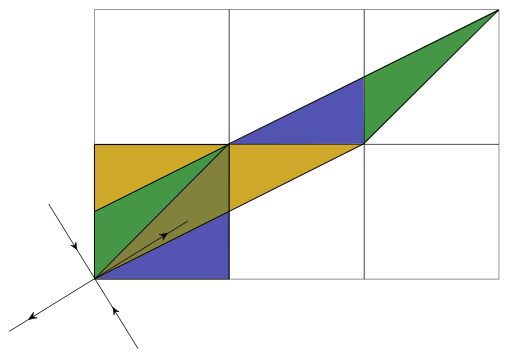
\includegraphics[scale=0.5]{Arnoldcatmap.png}
	\caption{The lines with the arrows show the contracting and expanding eigenspaces. The control should force the state to straddle the contracting eigenspaces to reach the hyperbolic equilibrium point.  \texttt{https://commons.wikimedia.org/wiki/File:Arnoldcatmap.svg} }
\end{figure}
 State-action feature vector with tile coding $x = x(s, a)$ is used to encode the 2-dimensional continuous state space $[-2, 2] \times [-2, 2] \subset \mathbb{R}^2$. 10 tilings were used with tile width $= [0.1, 0.1]$. The actions were parametrized to limit the control to act only in the $x$-direction with the options being move left, right, and no control with corresponding control vectors being $[-1, 0], [1, 0], [0,0]$. The Q-function is then parametrized as $q(s, a, w) = w^Tx(s,a)$. 
 
The initial condition was chosen to be within a 2-D ball of radius 0.05 centered at $[-1.62, 1]$ which lies on the contracting eigenspace. The terminal states are the cases where the state reaches failure regions defined to be $b$ away from the contracting eigenspaces (below the line $y = \dfrac{-2x}{1+\sqrt{5}} - b$ and above the line $y = \dfrac{-2x}{1+\sqrt{5}} + b$). Refer to figure \label{fig:o_control} for details. If the controller is successful in containing the state to be within the success region for 400 time steps, a terminal state is reached. For each time step in the success region, a reward of $+1$ is received. A controller which always moves in the direction of the contracting eigenspace is able to achieve this goal given sufficiently small process noise. 


\begin{figure}[H]
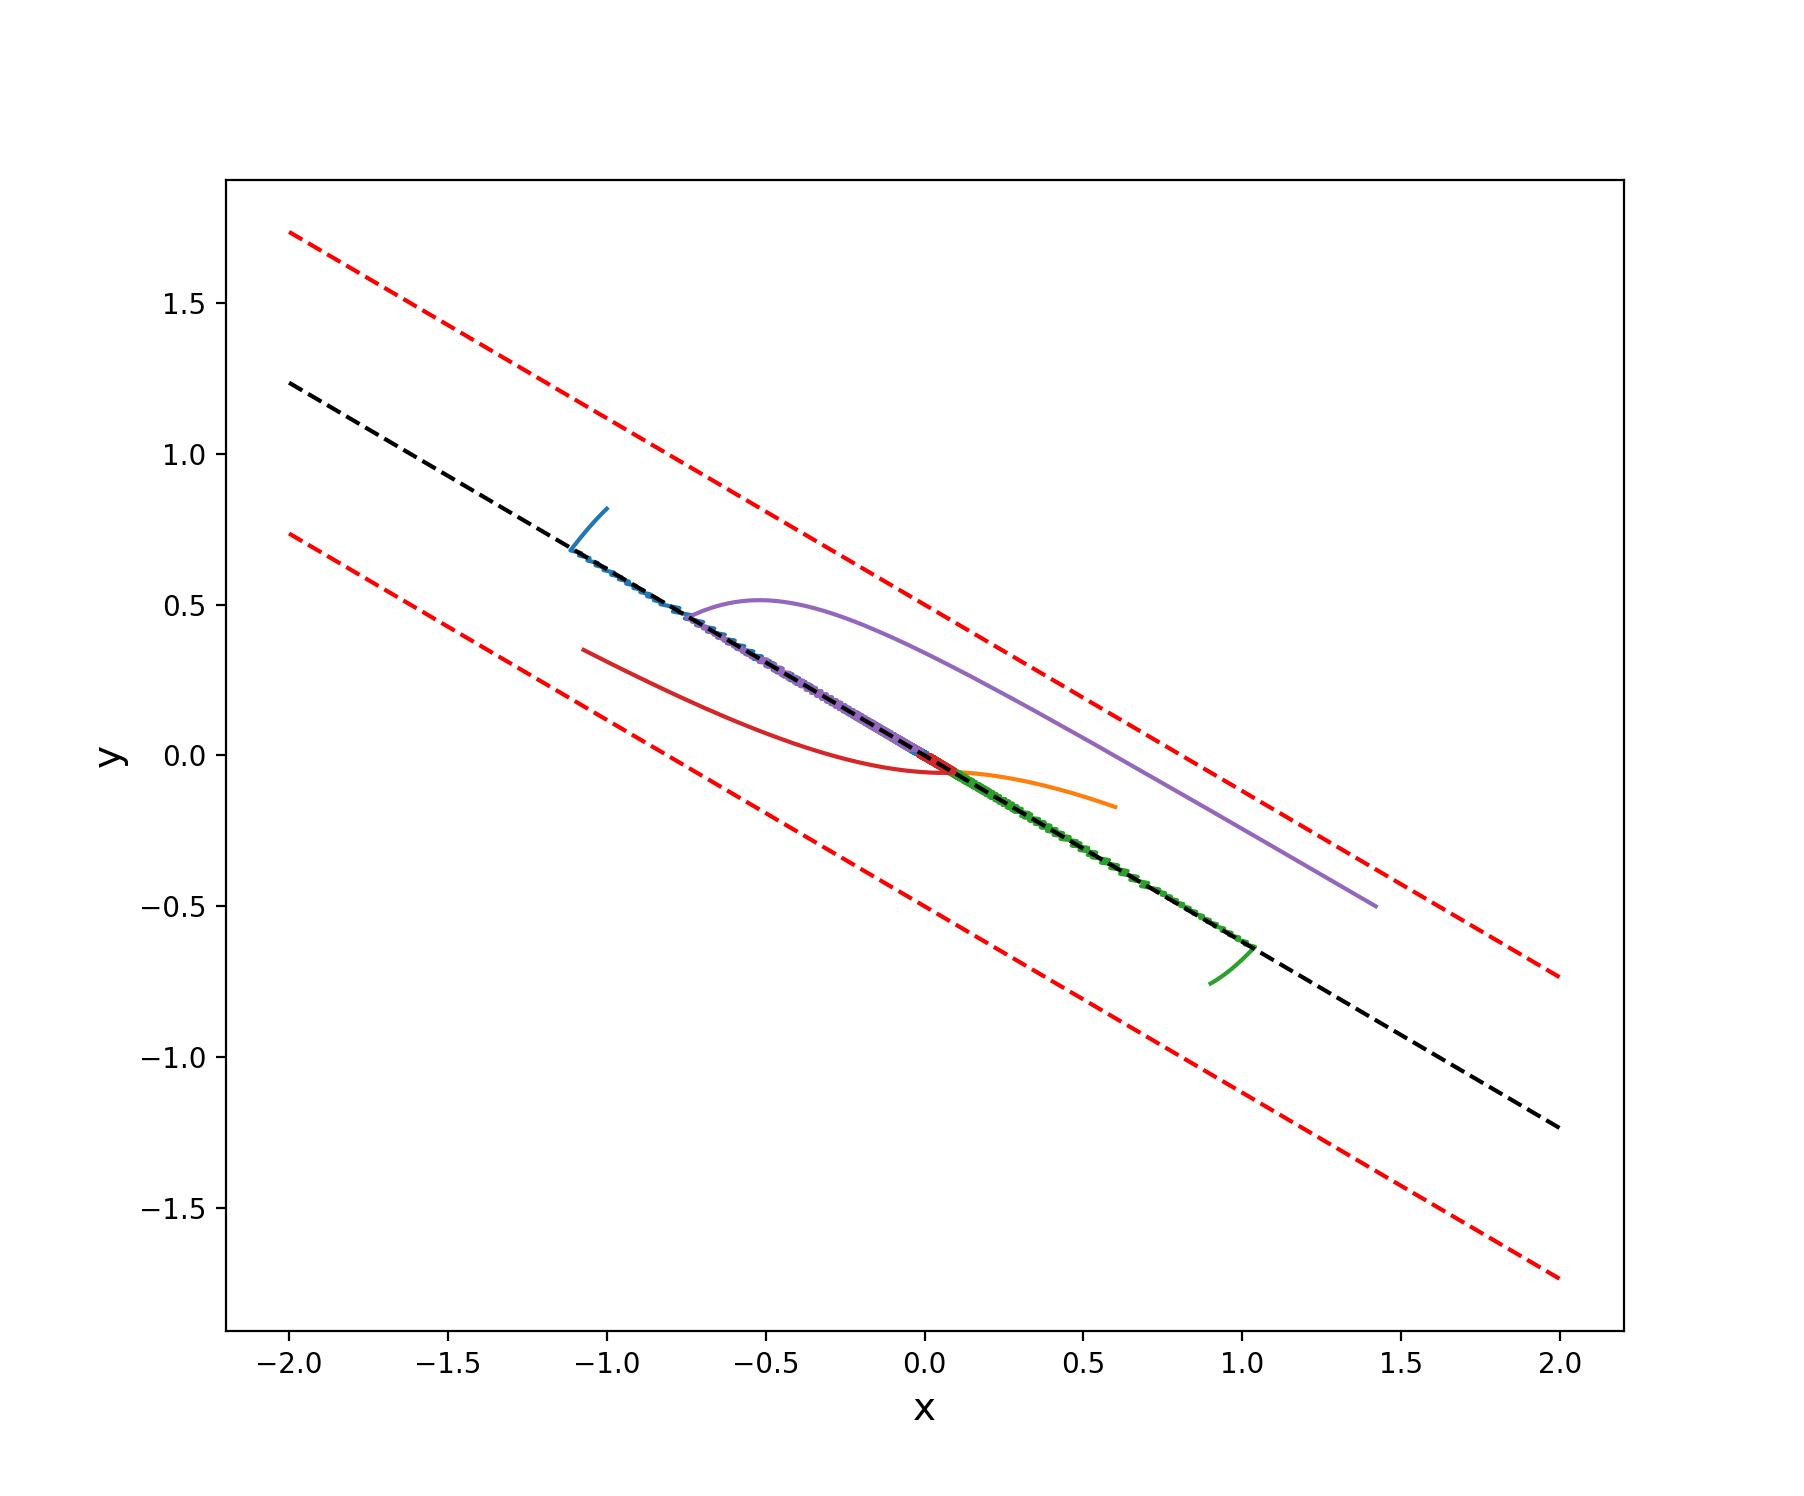
\includegraphics[scale=0.5]{optimal_controller.png}
\label{fig:o_control}
\caption{The red dotted-lines indicate the regions bounding successful control. The black dotted-line denotes the contracting eigenspace. The paths generated by the controller always moving in the direction of the contracting eigenspace is shown.}
\end{figure}

The following illustrates the results of the above described control problem using True online Sarsa($\lambda$) for increasing measurement noise. All other parameters kept constant across trials. For each trial, True online Sarsa ($\lambda$) uses 2000 episodes to learn $q_*$. For control \textit{without} Kalman filtering, the feature function is defined from $x : \mathcal{Z}^+ \times \mathcal A \rightarrow \mathbb{R}^d$ where $\mathcal{Z}$ is the measurement space including the terminal state. For control \textit{with} Kalman filtering, the feature function is defined as usual: $x : \mathcal{S}^+ \times \mathcal A \rightarrow \mathbb{R}^d$. The learned $w$ for the parametrized policy is then evaluated using the average reward over 100 control trials with the initial state chosen to be randomly within a 2-D ball of radius 0.05 centered at $[-1.62, 1]$. Figure (\ref{fig:kf_control}) shows that Kalman filtering based estimation of state enables True online Sarsa($\lambda$) to effectively learn a controller under process and measurements noise. The difference in performance is drastic as the measurement noise reaches the magnitude of the control.

\begin{figure}[H]
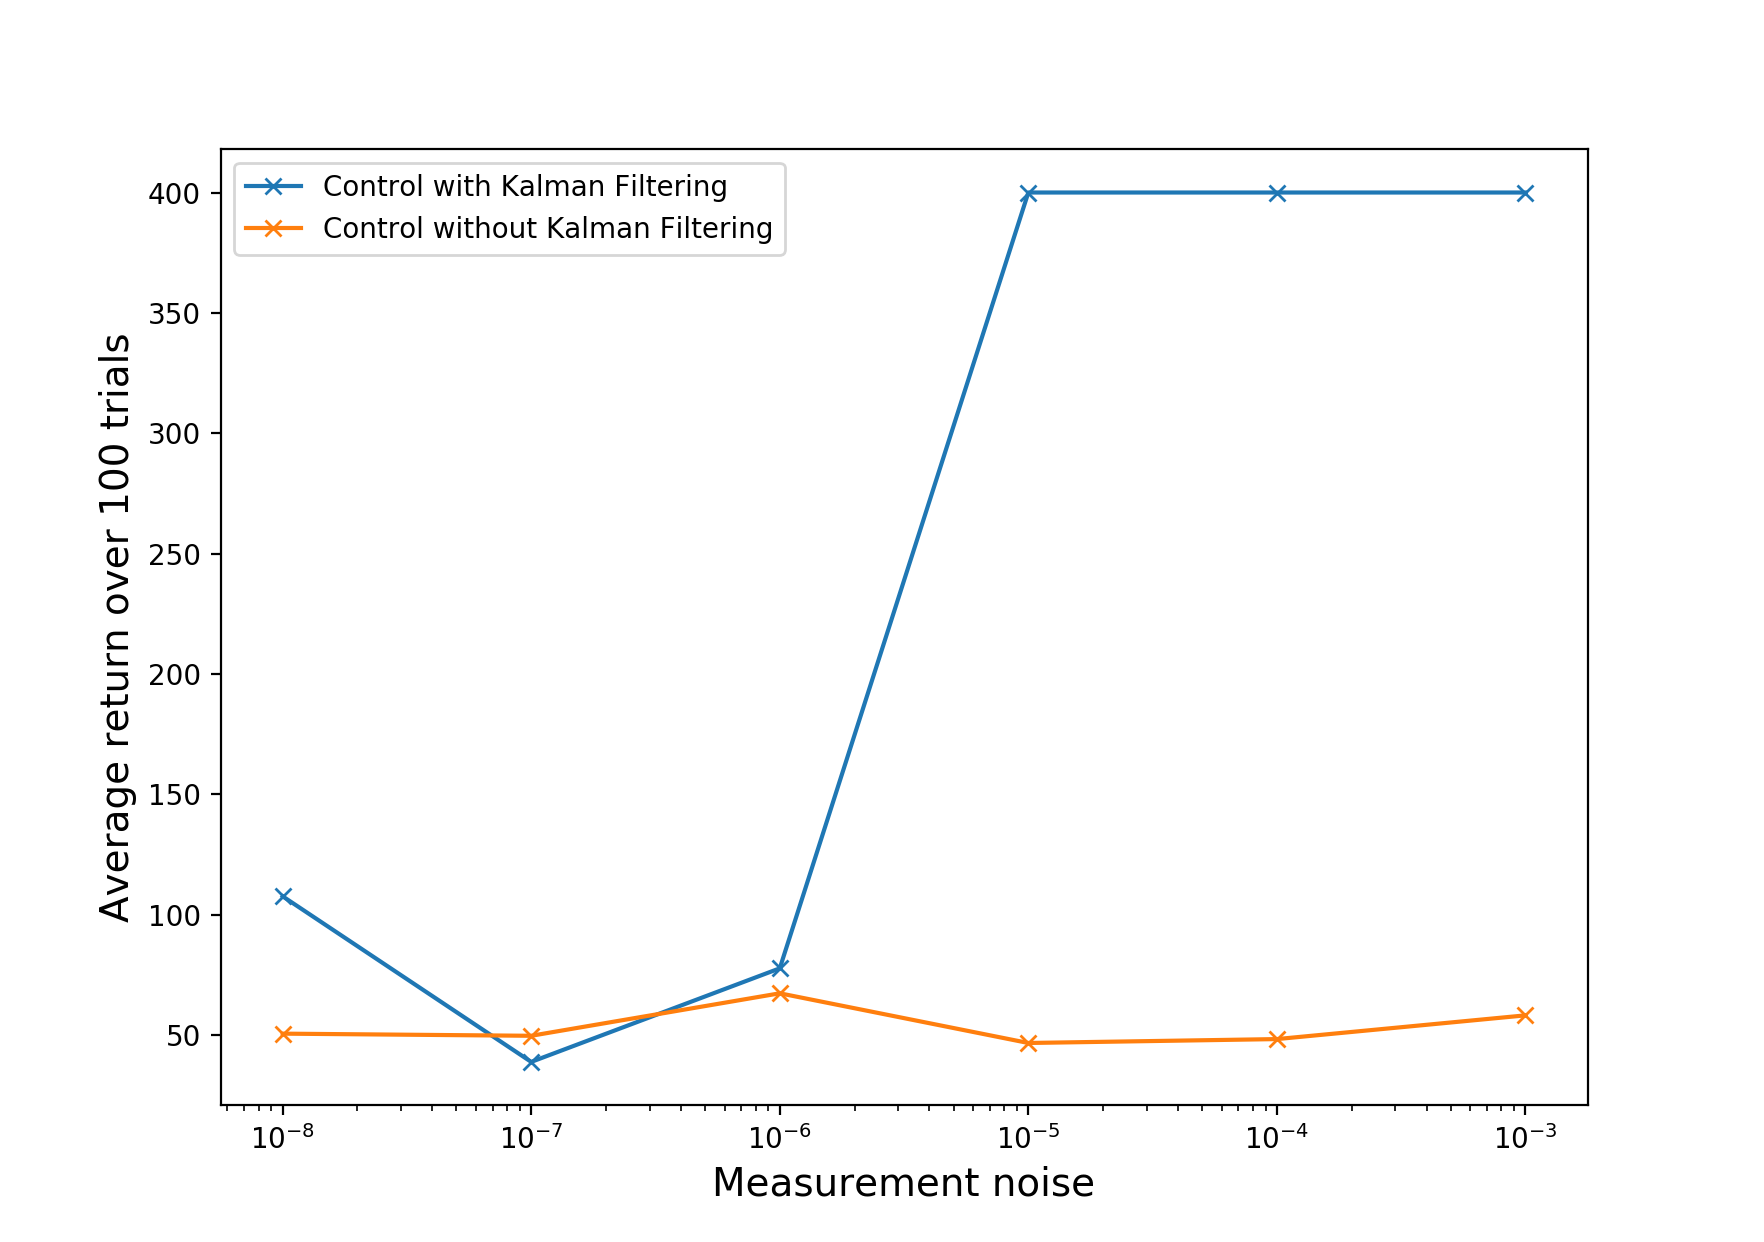
\includegraphics[scale=0.5]{2d_res.png}
\label{fig:kf_control}
\caption{Comparison of $q_*$ obtained with Kalman filtering state estimation vs using only measurements.}
\end{figure}



\bibliographystyle{plain} 
\bibliography{references}

\end{document}
